\documentclass[10pt,a4paper]{article}
\usepackage[T1]{fontenc}
\usepackage{lmodern,microtype,graphicx,xcolor,fancyhdr,listings,hyperref}
\usepackage[margin=16mm,top=15mm,bottom=17mm,footskip=8mm]{geometry}
\graphicspath{{screenshots/}{docs/screenshots/}}
\definecolor{ink}{HTML}{193448}\definecolor{accent}{HTML}{00665D}\definecolor{pale}{HTML}{EFF5F4}
\hypersetup{pdftitle={Sonne: automatic installation with Autodesk},colorlinks=true,urlcolor=accent}
\renewcommand{\familydefault}{\sfdefault}
\pagestyle{fancy}\fancyhf{}\renewcommand{\headrulewidth}{0pt}
\fancyfoot[L]{\small River Team / Sonne setup}\fancyfoot[R]{\small\thepage}
\setlength{\parindent}{0pt}\setlength{\parskip}{4pt}
\lstset{basicstyle=\ttfamily\small,backgroundcolor=\color{pale},columns=fullflexible,keepspaces=true,showstringspaces=false,aboveskip=3pt,belowskip=3pt}
\newcommand{\heading}[1]{\pdfbookmark[0]{#1}{setup-\thepage}{\LARGE\bfseries\color{ink}#1}\par\smallskip}
\newcommand{\step}[1]{\par\smallskip{\bfseries\color{accent}#1}\par}
\newcommand{\go}{\,$\rightarrow$\,}
\newcommand{\pic}[3]{\includegraphics[width=#2,height=#3,keepaspectratio]{autodesk/#1.png}}
\newcommand{\sources}[1]{\vfill{\scriptsize Screenshot credits: #1}\par}
\begin{document}
\heading{1. Create the Forma project}
\step{Autodesk Account / Create the hub}
Sign in as team administrator. Open \textbf{Products and services \go Hubs \go Create hub \go Forma}. Enter a hub name, select the team and region, then click \textbf{Create hub}. Keep the region for setup. Add an administrator or click \textbf{Skip}, then open the hub.
\begin{center}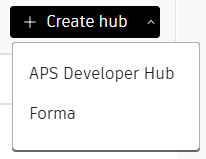
\includegraphics[width=27mm]{forma-hub-menu.png}\hfill\pic{hub-fields}{50mm}{36mm}\hfill\pic{hub-admin}{40mm}{31mm}\hfill\pic{hub-open}{44mm}{31mm}\end{center}
\step{Forma / Create the project and add the Revit user}
Click \textbf{Create project}. Enter \texttt{Sonne Pilot}, select the hub and project type, then confirm. In \textbf{Project Admin \go Members \go Add members}, enter the Revit user's email and grant Data Management access.
\begin{center}\pic{project-list}{36mm}{30mm}\hfill\pic{project-form}{52mm}{36mm}\hfill\pic{members}{60mm}{36mm}\end{center}
\step{Data Management / Set folder permissions}
In \textbf{Files}, open the \textbf{Project Files} menu (\ldots) \go \textbf{Add subfolder}. Name it \texttt{Sonne Test}. Open its menu \go \textbf{Permissions settings \go Add}. Select the Revit user, choose \textbf{Edit} and save.
\begin{center}\pic{subfolder}{52mm}{24mm}\hfill\pic{permission-menu}{50mm}{22mm}\hfill\pic{edit}{60mm}{20mm}\end{center}
\step{Autodesk Account / Assign cloud worksharing}
\textbf{User Management \go By Product \go Revit Cloud Worksharing \go Assign users}. Select the team and assign the Revit user's email.
\begin{center}\pic{account-navigation}{100mm}{10mm}\end{center}
\sources{River Team capture; \href{https://help.autodesk.com/cloudhelp/ENU/Docs-Trials-Subscriptions/files/Purchase_And_Activate_Account.html}{Autodesk hub wizard};
\href{https://hdot.wiki/wp-content/uploads/2025/06/Creating-a-New-Project-and-Intial-Project-Settings-in-ACC-BPG-20230802-PDF.pdf}{HDOT project guide};
\href{https://resources.imaginit.com/autodesk-forma-formerly-autodesk-construction-cloud/adding-bulk-members-to-the-autodesk-forma-project}{IMAGINiT members};
\href{https://static.au-uw2-prd.autodesk.com/Class_Handout_CES500123_ClassHandout-CES500123-Smith-AU2021.pdf}{Autodesk University folders};
\href{https://help.autodesk.com/view/DOCS/ENU/?guid=Folder_Permissions}{Autodesk permissions}.}
\newpage
\heading{2. Connect Sonne to Autodesk}
\step{APS Developer Hub / Create the app}
\textbf{Applications \go Create application}. Enter \texttt{Sonne ACC Test}, select \textbf{Traditional Web App} and click \textbf{Create}.
\begin{center}\pic{apps}{55mm}{28mm}\hspace{10mm}\pic{app-type}{75mm}{47mm}\end{center}
\step{App settings / Register the callback}
Paste this URL in \textbf{Callback URLs}. Under \textbf{API Access}, enable \textbf{Data Management}, \textbf{Forma APIs} and \textbf{Webhooks}. Click \textbf{Save changes}.
\begin{lstlisting}
http://localhost:8765/aps/oauth/callback
\end{lstlisting}
\begin{center}\pic{callback}{88mm}{43mm}\hfill\pic{credentials}{78mm}{30mm}\end{center}
Copy the \textbf{Client ID} for the hub integration. Keep the \textbf{Client Secret} for the installer.
\step{Forma Hub Admin / Add the integration}
\textbf{Custom integrations \go Add custom integration}. Enter the Client ID, app name and description. Click \textbf{Next}. If using a Secure Service Account, invite it to the project. In a dedicated test hub without one, \textbf{Proceed anyway} grants hub-wide access. Confirm the status is \textbf{Active}.
\begin{center}\pic{custom}{67mm}{46mm}\hspace{12mm}\pic{integration}{65mm}{46mm}\end{center}
\sources{\href{https://get-started.aps.autodesk.com/}{Autodesk APS Getting Started};
\href{https://help.autodesk.com/cloudhelp/ENU/Docs-Admin/files/hub-administration/Custom_Integrations.html}{Autodesk custom integrations}.}
\newpage
\heading{3. Publish the model and run setup}
\step{Revit 2027 / Publish the baseline}
Open the test RVT as the enrolled project user. Rename the existing schedule containing SNE-1 and SNE-2 to \texttt{Test Rooms-Sonne}. Select \textbf{Collaborate \go Collaborate \go In the cloud \go OK}. Save in \textbf{Sonne Pilot \go Project Files \go Sonne Test}.
\begin{center}\pic{collaborate}{40mm}{34mm}\hfill\pic{save-model}{56mm}{34mm}\hfill\pic{publish}{31mm}{34mm}\hfill\pic{acc-files}{42mm}{30mm}\end{center}
In \textbf{Revit Home \go Autodesk Projects}, open the model menu (\ldots) \go \textbf{Publish Latest} if pending. In ACC Files, open the published model or its folder and copy the browser URL.
\step{Sonne server / Run the automatic installer}
On the River Team PC, enter \texttt{wsl -u river} in Windows PowerShell. In WSL run:
\begin{lstlisting}
cd /mnt/c/Users/sperm/Documents/ChatGPT/riverteam/Sonne
bash scripts/install-sonne.sh --with-acc
\end{lstlisting}
For a remote server, connect with \texttt{ssh -L 8765:127.0.0.1:8765 user@server} and run the installer from its Sonne checkout. Keep SSH open during sign-in.
\par\textbf{Model and Discord} \quad Choose Qwen (12~GiB host RAM) or Gemma (16~GiB). On first install, enter the bot token, Discord OAuth2 secret, application, server, channel and user IDs, and Prompt Studio URL.
\par\textbf{Revit router} \quad Enter the workstation-facing HTTPS URL ending in \texttt{/revit/}, or press Enter to reuse the saved URL.
\par\textbf{Autodesk} \quad Enter the ACC URL, hub region, APS Client ID and secret. If prompted, enter the RVT filename. Open the printed sign-in link and approve read access with the project user's account.
\begin{center}\pic{authorize}{63mm}{32mm}\end{center}
\step{Windows workstation / Connect the client}
WSL sets up the client configuration in the Windows Sonne folder automatically. For a separate server, privately transfer the enrollment file printed by setup to \path{.state/revit-client/config.json} in the workstation's Sonne folder.

For a new client, close Revit. From the Windows Sonne folder, run:
\begin{lstlisting}
.\scripts\install-revit-client.cmd
\end{lstlisting}
Reopen the cloud model. Start the client from the same checkout:
\begin{lstlisting}
.\scripts\start-revit-client.cmd
\end{lstlisting}
\textbf{Ready:} \texttt{ACC mode is running} and a baseline version appear in the setup terminal. Leave the terminal and client running for alerts.
\sources{\href{https://files.upskill-dev.autodesk.com/public/aex/bim/bimaeco/pdf/BIMAECO_PE_M3_Collaborate-with-a-cloud-workshared-central-model.pdf}{Autodesk cloud worksharing exercise};
\href{https://www.autodesk.com/support/technical/article/caas/sfdcarticles/sfdcarticles/How-to-publish-latest-Cloud-Models-using-the-New-Revit-Home-interface.html}{Autodesk Publish Latest};
\href{https://help.autodesk.com/cloudhelp/ENU/Docs-Files/files/File_Folder_Actions_Docs.html}{Autodesk Files}, \href{https://aps.autodesk.com/en/docs/oauth/v2/overview/scopes}{Autodesk authorization scopes};
\href{https://static.au-uw2-prd.autodesk.com/Class_Presentation_FDC122160_Seamless_integration_with_Forge_Webhooks_Adam_Nagy_1.pdf}{Autodesk University consent example}.}
\end{document}
